% LaTeX template for academic reports (thesis)

\documentclass[12pt,english,a4paper,oneside]{article}
\let\circledS\undefined
\usepackage{setspace}
\setstretch{2.0}
\usepackage{amssymb,amsmath}
\usepackage{ifxetex,ifluatex}
\usepackage[nottoc]{tocbibind}
\usepackage{csquotes}
\usepackage[usenames,dvipsnames]{xcolor}
\usepackage[bookmarks, colorlinks, breaklinks]{hyperref}
\definecolor{mannheimblue}{HTML}{003056}
\definecolor{mannheimorange}{HTML}{df7e50}

\hypersetup{linkcolor=mannheimblue,
citecolor=mannheimblue,
filecolor=black,
urlcolor=mannheimblue}


% some more packages...
\usepackage{graphicx}
%\usepackage{scrpage2}
%\usepackage{xcolor}
\usepackage{hyperref}
%\hypersetup{colorlinks=true, linkcolor = blue, urlcolor = blue}
%\usepackage{eso-pic}

\renewenvironment{quote}{\list{}\item\relax
\small\singlespacing}{\endlist}
\SetBlockEnvironment{quote}

\onehalfspacing
% \renewcommand{\baselinestretch}{1.5}  % line distance is 1.5

%\renewcommand{\chaptername}{} %% remove the word \chapter

% % \newlength{\cslhangindent}
% \setlength{\cslhangindent}{1.5em}
% \newenvironment{CSLReferences}%
%   {\setlength{\parindent}{0pt}%
%   \everypar{\setlength{\hangindent}{\cslhangindent}}\ignorespaces}%
%   {\par}
% 
% Pandoc citation processing
\newlength{\cslhangindent}
\setlength{\cslhangindent}{1.5em}
\newlength{\csllabelwidth}
\setlength{\csllabelwidth}{3em}
\newlength{\cslentryspacingunit} % times entry-spacing
\setlength{\cslentryspacingunit}{\parskip}
% for Pandoc 2.8 to 2.10.1
\newenvironment{cslreferences}%
  {\setlength{\parindent}{0pt}%
  \everypar{\setlength{\hangindent}{\cslhangindent}}\ignorespaces}%
  {\par}
% For Pandoc 2.11+
\newenvironment{CSLReferences}[2] % #1 hanging-ident, #2 entry spacing
 {% don't indent paragraphs
  \setlength{\parindent}{0pt}
  % turn on hanging indent if param 1 is 1
  \ifodd #1
  \let\oldpar\par
  \def\par{\hangindent=\cslhangindent\oldpar}
  \fi
  % set entry spacing
  \setlength{\parskip}{#2\cslentryspacingunit}
 }%
 {}
\usepackage{calc}
\newcommand{\CSLBlock}[1]{#1\hfill\break}
\newcommand{\CSLLeftMargin}[1]{\parbox[t]{\csllabelwidth}{#1}}
\newcommand{\CSLRightInline}[1]{\parbox[t]{\linewidth - \csllabelwidth}{#1}\break}
\newcommand{\CSLIndent}[1]{\hspace{\cslhangindent}#1}
% % \newlength{\cslhangindent}
% \setlength{\cslhangindent}{1.5em}
% \newlength{\csllabelwidth}
% \setlength{\csllabelwidth}{3em}
% \newenvironment{CSLReferences}[3] % #1 hanging-ident, #2 entry spacing
%  {% don't indent paragraphs
%   \setlength{\parindent}{0pt}
%   % turn on hanging indent if param 1 is 1
%   \ifodd #1 \everypar{\setlength{\hangindent}{\cslhangindent}}\ignorespaces\fi
%   % set entry spacing
%   \ifnum #2 > 0
%   \setlength{\parskip}{#2\baselineskip}
%   \fi
%  }%
%  {}
% \usepackage{calc} % for \widthof, \maxof
% \newcommand{\CSLBlock}[1]{#1\hfill\break}
% \newcommand{\CSLLeftMargin}[1]{\parbox[t]{\maxof{\widthof{#1}}{\csllabelwidth}}{#1}}
% \newcommand{\CSLRightInline}[1]{\parbox[t]{\linewidth}{#1}}
% \newcommand{\CSLIndent}[1]{\hspace{\cslhangindent}#1}
% 
\usepackage{fixltx2e} % provides \textsubscript
\ifnum 0\ifxetex 1\fi\ifluatex 1\fi=0 % if pdftex
  \usepackage[T1]{fontenc}
  \usepackage[utf8]{inputenc}
\else % if luatex or xelatex
  \ifxetex
    \usepackage{mathspec}
  \else
    \usepackage{fontspec}
  \fi
  \defaultfontfeatures{Ligatures=TeX,Scale=MatchLowercase}

\fi
% % use upquote if available, for straight quotes in verbatim environments
% \IfFileExists{upquote.sty}{\usepackage{upquote}}{}
% % use microtype if available
% \IfFileExists{microtype.sty}{%
% \usepackage{microtype}
% \UseMicrotypeSet[protrusion]{basicmath} % disable protrusion for tt fonts
% }{}
% % \usepackage[left=2.5cm,right=2.5cm,top=2.5cm,bottom=2.5cm]{geometry}
% \usepackage{hyperref}
\hypersetup{unicode=true,
            pdftitle={On Using the Metropolis-Hastings Algorithm for Data Imputation},
            pdfauthor={Tobias Stenzel},
            pdfborder={0 0 0},
            breaklinks=true}
\urlstyle{same}  % don't use monospace font for urls
\ifnum 0\ifxetex 1\fi\ifluatex 1\fi=0 % if pdftex
  \usepackage[shorthands=off,main=english]{babel}
\else
  \usepackage{polyglossia}
  \setmainlanguage[]{english}
\fi
% % \usepackage{longtable,booktabs}
\setlength{\emergencystretch}{3em}  % prevent overfull lines
\providecommand{\tightlist}{%
  \setlength{\itemsep}{0pt}\setlength{\parskip}{0pt}}
\setcounter{secnumdepth}{5}
% Redefines (sub)paragraphs to behave more like sections
\ifx\paragraph\undefined\else
\let\oldparagraph\paragraph
\renewcommand{\paragraph}[1]{\oldparagraph{#1}\mbox{}}
\fi
\ifx\subparagraph\undefined\else
\let\oldsubparagraph\subparagraph
\renewcommand{\subparagraph}[1]{\oldsubparagraph{#1}\mbox{}}
\fi


\usepackage{csquotes}
\usepackage{fancyhdr} % to change header and footers
\usepackage{url}
\def\UrlBreaks{\do\/\do-}

%%%% plagiarism

\newcommand*{\SignatureAndDate}[1]{%
\vspace{2cm}
     Mannheim, den \makebox[2cm]{\hrulefill} \hfill\makebox[9cm]{\hrulefill}%
     \par
%  \makebox[2cm]{ Ort, Datum}
  \hfill\makebox[7.5cm][t]{Name und Unterschrift}
  \vspace{2cm}
}%

 \newcommand*{\SignatureAndDateEng}[1]{%
\vspace{2cm}
     Mannheim, \makebox[2cm]{\hrulefill} \hfill\makebox[9cm]{\hrulefill}%
     \par
    \hfill\makebox[7.5cm][t]{Name and Signature}%
\vspace{2cm}
}%


\makeatletter
\newenvironment{kframe}{%
\medskip{}
\setlength{\fboxsep}{.8em}
 \def\at@end@of@kframe{}%
 \ifinner\ifhmode%
  \def\at@end@of@kframe{\end{minipage}}%
  \begin{minipage}{\columnwidth}%
 \fi\fi%
 \def\FrameCommand##1{\hskip\@totalleftmargin \hskip-\fboxsep
 \colorbox{shadecolor}{##1}\hskip-\fboxsep
     % There is no \\@totalrightmargin, so:
     \hskip-\linewidth \hskip-\@totalleftmargin \hskip\columnwidth}%
 \MakeFramed {\advance\hsize-\width
   \@totalleftmargin\z@ \linewidth\hsize
   \@setminipage}}%
 {\par\unskip\endMakeFramed%
 \at@end@of@kframe}
\makeatother

%\renewenvironment{Shaded}{\begin{kframe}}{\end{kframe}} ses 2019-03-08












\newcommand{\ts}{\thinspace}



\usepackage{tikz, float, caption, amsthm, algorithm, algpseudocode}
\floatplacement{figure}{H}
\interfootnotelinepenalty=10000

%% font EB Garamond
\setmainfont[
Path = fonts/static/,
BoldFont = EBGaramond-Bold.ttf,
ItalicFont = EBGaramond-Italic.ttf,
BoldItalicFont  = EBGaramond-BoldItalic.ttf]
{EBGaramond-Regular.ttf}


% \usepackage{float}

\usepackage{amsthm}
\newtheorem{theorem}{Theorem}[section]
\newtheorem{lemma}{Lemma}[section]
\newtheorem{corollary}{Corollary}[section]
\newtheorem{proposition}{Proposition}[section]
\newtheorem{conjecture}{Conjecture}[section]
\theoremstyle{definition}
\newtheorem{definition}{Definition}[section]
\theoremstyle{definition}
\newtheorem{example}{Example}[section]
\theoremstyle{definition}
\newtheorem{exercise}{Exercise}[section]
\theoremstyle{definition}
\newtheorem{hypothesis}{Hypothesis}[section]
\theoremstyle{remark}
\newtheorem*{remark}{Remark}
\newtheorem*{solution}{Solution}
\begin{document}  %%%%%%% main document %%%%%%%%%%%%%%%
\begin{titlepage}

    \begin{center}
    \large{ \textsc{ \uppercase{University of Mannheim} \\ \vspace{-0.2cm}
School of Social Sciences \\ \vspace{-0.2cm}
Department of Political Science}}

      
        \vspace{3.5cm}
        

       \large{   Final Paper for Course   }


       \large{ \textit{   Advanced Quantitative Methods in Political Science   }}

\renewcommand{\linethickness}{0.03em}
\rule{\linewidth}{\linethickness}


       \LARGE{ \textbf{   On Using the Metropolis-Hastings Algorithm for Data Imputation   }}

        % \vspace{-0.5cm}

       \large{  }

        \vspace{-0.2cm}
\rule{\linewidth}{\linethickness}


\begin{minipage}[t]{0.5\textwidth}
\begin{flushleft}
\singlespacing
 \textbf{Tobias Stenzel}  \\ 


 \href{mailto:tobias.stenzel@students.uni-mannheim.de}{\nolinkurl{tobias.stenzel@students.uni-mannheim.de}}  \\ 

\end{flushleft}
\end{minipage}
\begin{minipage}[t]{0.4\textwidth}
\hfill
\end{minipage}\\
\vspace{0.2cm}
\begin{minipage}[t]{0.35\textwidth}
\hfill
\end{minipage}
\begin{minipage}[t]{0.55\textwidth}
\begin{flushright}
\singlespacing
     Prof.~Thomas Gschwend, Ph.D.  \\       

\end{flushright}
\end{minipage}\\
%


         \vfill
         Submission Date: Mai 18, 2022 \\ 
        





         \vfill



     \end{center}
    \thispagestyle{empty}
\end{titlepage}

\newpage
% \thispagestyle{empty}
% \mbox{}







{
\setcounter{tocdepth}{2}
\newpage
\pagenumbering{gobble}
\tableofcontents
}

\newpage
\pagenumbering{arabic}
\fancypagestyle{plain}{%
    \renewcommand{\headrulewidth}{0pt}%
    \fancyhf{}%
    \fancyfoot[R]{\thepage}%
}
% Set the right side of the footer to be the page number
\pagestyle{plain}
\hypertarget{introduction}{%
\section{Introduction}\label{introduction}}

In recent years scholars have found declining support for democracy in long-established democracies. (Denemark et al. 2016; Foa and Mounk 2016, 2017; Norris 2017; Voeten 2016). This finding raises two important questions: First, what are the reasons for this decline, and second, what are its implications, i.e., does a decline in democratic support endanger the survival of these democracies?

A series of recent articles (Claassen 2019, 2020a, 2020b) researches these questions and presents novel results. Regarding the first question, Claassen (2020a) finds -- in contrary to the the widely held belief of self-reinforcing democracies -- that democratic support naturally fluctuates over time. The reasons is that increases in democracy levels lead to decreases in public support and vice versa. Regarding question two, so far the results about the relationship between democratic support and its survival have been mixed. Claassen (2020a), however, finds supporting evidence for the natural theory that democratic support plays a positive role in the system's survival.

A main obstacle for researching democratic support is that current panel data contains a large number of missing values. Claassen (2019) finds an approach to simulate dense panel data from the actual fractured data. The two most recent studies both rely on this data. His approach consists of three steps: First, assume a probabilistic structural model of democratic support. Second, estimate its parameters via the Metropolis Hastings algorithm using the fractured data. Third, simulate the data using the model and the large number of parameter estimates.

The objective of this work is to evaluate the robustness of Claassen's findings towards changes in the method's hyperparameters. In other words, I incorparate the uncertainty about the right choice of hyperparameters into Claassen's results to test their reliability. In particular, I propagate a random set of hyperparameters through Claassen's estimation procedure. This is important because arbitrary hyperparameter choices can potentially lead to false or at least random results. Therefore, the respective parametric uncertainty should always be reported along the point estimate.

I come to the following results:

The final paper is structured as follows: Section 2 reviews the literature of public support with a focus on Claassen's papers and defines the concept. Section 3 explains Claassen's model of public support, its estimation and my approach for the uncertainty propagation. Section 4 presents the results and Section 5 discusses the findings. Section 6 concludes.

\hypertarget{literature-review-and-data}{%
\section{Literature Review and Data}\label{literature-review-and-data}}

\hypertarget{the-concept-of-democratic-support}{%
\subsection{The Concept of Democratic Support}\label{the-concept-of-democratic-support}}

There are two major conceptualizations of public support for democracy (PSD). First, the \enquote{implicit} approach that requires the support for broader sociopolitical values like post-materialism and egalitarianism. Here, people support democracy implicitly if they support the values that are framed as particularly democratic. Second, the \enquote{explicit} approach that requires both an appraisal of democracy and a rejection of autocratic alternatives. Some studies also refer to PSD measured on the national level as \enquote{mood.}

\hypertarget{drivers-of-democratic-support}{%
\subsection{Drivers of Democratic Support}\label{drivers-of-democratic-support}}

The main theory about why citizen and societies begin to support democracy are called \emph{generational socialization} and \emph{instrumental regime performance}. The first theory assumes that individuals are taught to support the regime under which they are socialized during late adolescence (Mannheim 1970; Niemi 1974). One implication is that after a shift to democracy, the support for it will grow over time (Denemark et al. (2016)). Indeed, several single-country studies have found evidence for this claim, for example for 1970s Germany (Baker et al. (1981)), 1980s Spain (Montero, Gunther, and Torcal (1997)), and 1990s Russia (Mishler and Rose (2007)). One the other hand, other studies do not find such an effect analyzing other Central and Eastern European countries (Mishler and Rose (2002)). Furthermore, more recent studies even find a decline in PSD over the last years (Foa and Mounk 2016, 2017).

Regarding the second theory, instrumental regime performance, PSD rises if the system performs well in terms of instrumental benefits such as economic growth and it declines if the opposite is the case (Dalton 1994; Magalhães 2014). Consequently, the theory suggests that during PSD declines during economic crises. However, there are case-studies that do (Dalton 1994; Magalhães 2014; Mishler and Rose 1996) and that do not (Graham and Sukhtankar (2004)) find this relationship in the data.

Claassen (2020b) offers an alternative theory in transferring the thermostatic model of public opinion and policy (Wlezien (1995)) to democracy and democratic support. In particular, he suggests that there is a negative feedback loop between PSD and democracy so that PSD decreases if democracy supply increases and vice versa. In short, the reasoning is that the output of democratic rights and institutions overshoots the initial desire for them which causes another overcompensation in favor of lower levels of democracy. Moreover, Claassen (2020b) finds different causal channels for electoral and minoritarian democracies. These two sub-types differ in the degree to which the majority holds juridical power. Therefore, he tests the following hypotheses: First, increases in democracy have a negative effect on PSD (H1), Second, he specifically looks at electoral (H1-elec) and minoritarian democracies (H1-min). In his analysis he finds evidence for H1 and H1-min but not for H1-elec.

\hypertarget{democratic-support-and-survival-of-democracy}{%
\subsection{Democratic Support and Survival of Democracy}\label{democratic-support-and-survival-of-democracy}}

Claassen (2020a) distinguishes between two types of PSD: diffuse and specific. Specific PSD is instrumental and focuses on regime outputs (similar to the instrumental regime performance theory), whereas diffuse support is normative and focuses on the principles of the regime. Therefore, principled PSD is more durable than specific support and helps cushioning regimes in times of political or economic crises. It is thus principled PSD that helps to ensure the survival of democracy. Although the theory is widely accepted (e.g., Norris (2017), Booth and Seligson (2009), Mattes and Bratton (2007)), the findings so far have also been mixed with supporting contributions (Inglehart 2003; Welzel and Inglehart 2005) and contributions against the theory (Fails and Pierce 2010; Hadenius and Teorell 2005; Qi and Shin 2011; Welzel 2007). Astonishingly, these studies essentially analyze the same data from the World Value Survey starting at wave 3 where respective PSD items are included.

Claassen (2020a) does not only look at the relationship between PSD and democractic survival but also between PSD and democratic emergence. He includes the argument made by Qi and Shin (2011) that PSD may also function as democratic demand, thus increasing the probability of transitioning from autocracy to democracy. Claassens hypotheses thus are: First, PSD is positively associated with subsequent change in democracy regardless of the initial level of democracy. Second, he specifically looks at PSD in already-existing democracies (H2-dem) and at PSD in autocracies (H2-aut). He finds evidence in support of H2-dem, mixed evidence for H2 and no evidence for H2-aut.

\hypertarget{measuring-democratic-support-and-the-data-challenge}{%
\subsection{Measuring Democratic Support and the Data Challenge}\label{measuring-democratic-support-and-the-data-challenge}}

We measure PSD with existing survey data on the national level. In particular, we focus on principled support. The questions ask for the respondent's opinion on the appropriateness or desirability of democracy and undemocratic alternatives and comparisons between both.\footnote{The 8 included survey items and their different variants can be found on \href{http://chrisclaassen.com/docs/Democratic_mood_supp_materials.pdf}{the author's webpage}.}

Such items are available in 14 survey projects,\footnote{World and European Values Surveys, the Afrobarometer, Arab Barometer, Latinobarometer, Asiabarometer, Asian Barometer, South Asia Barometer, New Europe Barometer, Latin American Public Opinion Project, Eurobarometer, European Social Survey, pew Global Attitudes Project, and the Comparative Study of Electoral Systems} for 150 countries, and from 1988 to 2017. Combined, the dataset includes 3,765 nationally aggregated binary responses from 1,390 nationally representative survey samples.

The data, however, poses the following challenge: It is highly fractured across time and space, with many -- oftentimes large -- gaps along the time dimension for all countries. Although we look at a 30 years time span, the average number of covered years is slightly below 8. For instance, China is the country with most participants over all years, namely 20895. However, from 1988 to 2020, the data available covers only 8 years: 2001-2003, 2006-2009, and 2011/2012. Many countries are not covered at all or only surveyed once. The South American countries, however, tend to have the best coverage. For instance, Argentina tops the list with 23 years included. Germany and the US are available for 12 and 13 years, respectively.

Figure \ref{fig:sparse-data} gives an overview of the sparseness of the data. The first panel shows the availability of at least one survey item across a selection of eight countries from 1990 to 2017. The other three panels focus on the three most common question themes. We see that the single item data is indeed sparse and that even the aggregated data contains lots of gaps.

\begin{figure}[H]
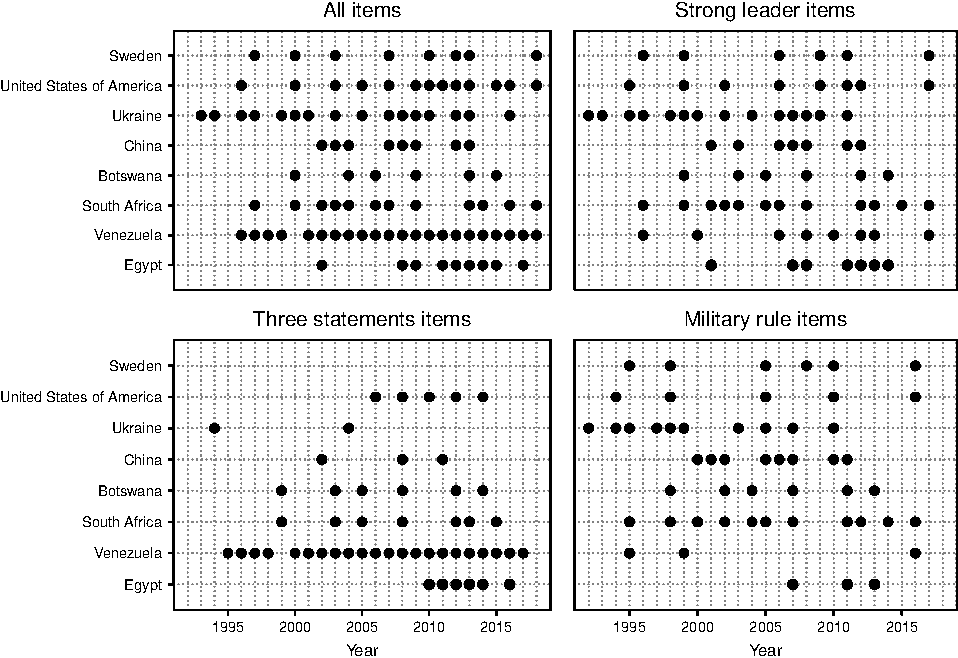
\includegraphics[width=\textwidth]{figs/sparse-data-1} \caption[Sparseness of Aggregate Support for Democacy By Country, Year, and Survey Item]{Sparseness of Aggregate Support for Democacy By Country, Year, and Survey Item. The figure is an update from Claassen (2019).}\label{fig:sparse-data}
\end{figure}

\noindent
So far, past research has responded to this issue by discarding most of the available data and using only small cross-sectional data sets consisting of data from only one survey project for one year (Inglehart 2003; Qi and Shin 2011; Welzel 2007). Of course, this leads to a disregard not only of all other countries but also of additional items. Claassen (2019) describes how to use most available data for simulating a dataset that is dense across the yearly time dimension. This dataset can then be used for subsequent statistical analyses (Claassen 2020a, 2020b). The next section describes Claassen (2019)'s approach.

\hypertarget{model-and-estimation}{%
\section{Model and Estimation}\label{model-and-estimation}}

Claassen (2019)'s approach for simulating dense panel data for PSD has the following three main steps: Step 1 is to define a sensible model of PSD item responses as a function of latent public opinion. Step 2 is to estimate the model parameters with the Metropolis Hastings Algorithm. Step 3 is to simulate the the data from the estimated model.

\hypertarget{the-latent-variable-model}{%
\subsection{The Latent Variable Model}\label{the-latent-variable-model}}

Claassen (2019) draws four principles from the literature to model cross-national timeseries for PSD: First, public opinion is an unobserved, latent trait that differs for each year and country. Then, each observed item response is a function of the latent trait. The function should therefore contain item-specific parameters to disaggregate the latent trait into multiple item responses and to account for heterogenuous item functioning. Second, estimating the latent variable from item-specific responses can be though of as \emph{smoothing} the opinion estimate over items since the latent variable does not contain this dimension. One should also smooth over the time dimension by not estimating the latent traits for each time period but rather by estimating the parameters that define a transitional model that holds for all periods. Third, we should not model the percentage of positive item responses but the number of positive and negative responses directly. With that, we can model the problem of smaller response samples. In the following I describe how Claassen (2019) incorporates these principles in the definition of his main model\footnote{The main model is called model 5 in Claassen (2019). It achieves lowest discrepancy between simulated and actual data and has the fifth highest complexity of six different specifications.} that we will call \(f\).\newline

\noindent
For each country \(i\), year \(t\), survey item \(k\), the number of positive answers is distrubted binomially with \(s\) as the number of total respondands and \(\pi\) as the probability of responding with yes.
\begin{equation}
\label{eq:num-resp}
y_{ikt} \sim \text{Binomial}(s_{ikt}, \pi_{ikt})
\end{equation}
We could now model \(\pi_{ikt}\) directly as a function of country-year and item-specific effects, \(\theta_{it}\) and \(\lambda_k\), respectively. However, we introduce additional dispersion by using another link function, the beta distribution to introduce additional dispersion. Survey data on public opinion are subject to various kinds of errors, for instance, translation, selection and interviewer mistakes. We model this error with the additional dispersion introduce by the beta distribution in Equation \eqref{eq:prob-yes}.

\begin{equation}
\label{eq:prob-yes}
\pi_{ikt} \sim \text{Beta}(\alpha_{ikt}, \pi_{ikt})
\end{equation}

\noindent
We reparametrize the two shape parameters \(\alpha\) and \(\beta\) to an expectation parameter \(\eta\) and a disperion paramter \(\phi\) in Equation \eqref{eq:expec} and \eqref{eq:dispersion}.

\begin{equation}
\label{eq:expec}
\alpha_{ikt} = \phi \eta_{ikt}
\end{equation}

\begin{equation}
\label{eq:dispersion}
\beta_{ikt} = \phi (1 - \eta_{ikt})
\end{equation}

\noindent
Now, we define the expectation of the number of positive responses per year, item and country as a function of item bias \(\lambda\), country-specific item bias \(\delta\) and latent, dynamic, country-specific PSD \(\theta\).

\begin{equation}
\label{eq:latent-country-year}
\eta_{ikt} = \text{logit}^{-1}(\lambda_k + \delta_{ik} + \theta_{it})
\end{equation}

\noindent
The item bias effect is distributed normally with expectation \(\mu_{\lambda}\) and variance \(\sigma_{\lambda}^2\).

\begin{equation}
\label{eq:item-intercept}
\lambda_k = \mathcal{N}(\mu_{\lambda}, \sigma_{\lambda}^2)
\end{equation}

\noindent
To model the heterogeneity of item country across item bias across countries (Stegmueller (2011)), we introduce the set of item by country effects \(\delta\).

\begin{equation}
\label{eq:country-effects}
\delta_k = \mathcal{N}(0, \sigma_{\delta}^2)
\end{equation}

\noindent
Our main parameter set, the latent parameters \(\theta\), capture the underlying time- and country-specific support for democracy. We fully capture the time dimension of the model by modeling the dynamics of \(\theta\) as an AR(1) process with normally distributed error term with variance \(\sigma_{\theta}^2\), zero intercept, and zero covariance as implied by Equation \eqref{eq:dynamics}.

\begin{equation}
\label{eq:dynamics}
\theta_{it} = \mathcal{N}(\theta_{i,t-1}, \sigma_{\theta}^2)
\end{equation}

\hypertarget{model-estimation-with-metropolis-hastings}{%
\subsection{Model Estimation with Metropolis-Hastings}\label{model-estimation-with-metropolis-hastings}}

One main application for the MH algorithm is Bayesian inference. Specifically, we want to estimate parameters \(\Theta\) of some probabilistic model \(f\). We have only limited prior knowledge of the distribution of \(\Theta\), for instance about its domain, that we use to define prior distributions \(p(\Theta)\). And we have a likelihood sample of \(f\) given the unknown \(\Theta\), namely \(p(y|\Theta)\). This would be our PSD data \(y_{ikt}\). We want use both, our prior knowledge and our data, to get our posterior distribution \(p(\Theta|y)\) in Equation \eqref{eq:bayes}. In this equation, posterior and likelihood are scaled by \(\frac{1}{p(y)}\). Without closed-form distributions, \(p(y)\) is usually unknown. This also implies that the posterior is proportional to the product of likelihood and prior.

\begin{equation}
\label{eq:bayes}
p(\Theta|y) = \frac{\mathcal{L}(y|\Theta)p(\Theta)}{p(y)} \propto \mathcal{L}(y|\Theta)p(\Theta)
\end{equation}

\noindent
An important insight is that our parameter vector \(\Theta\) does not only include
parameters defined as distributional means, for instance \(\theta\), but also
standard deviations like \(\sigma_{\theta}\). If our problem would not include those
variation parameters, a more direct option would be to solve \(\mathcal{L}(y|\Theta)p(\Theta)\) with the usual optimization algorithms. Those would
propose new values of \(\Theta\), evaluate its prior probability and the likelihood of
the data given \(\Theta\) until convergence and return the posterior mode or maximum a posteriori probability (MAP) estimate. Yet, since we need to estimate standard deviations,
we have to generate the whole parameter distributions to compute mean and variation. To this end, we use a Markov chain Monte Carlo (MCMC) method, namely the Metropolis Hastings algorithm.

Markov chains are stochastic processes that define distributions dependent on the values from only the previous period. The MH algorithm uses Markov chains to sample candidate parameters \(\Theta_i^*\) depending on \(\Theta_{i-1}\). For each candidate \(\Theta_i^*\), the algorithm uses the unscaled posterior, \(\mathcal{L}(y|\Theta_i)p(\Theta_i)\), and compares it with the posterior of \(\Theta_{i-1}\) (not requiring constant \(p(y)\)) to accept or reject new candidates. Comparing relative posterior probabilities thus allows us to sample from the posterior without knowing \(y\). The algorithm thus explores the domain proportionally to the posterior probability after a number of initial iterations. Besides the model specification using the MH algorithm requires the following choices: the choice of the prior distribution(s) \(p(\Theta)\), the choice of the proposal distribution \(g(y_i, y_{i-1})\), and the number of initial parameters to drop, i.e.~the length of the burnin-period. I include a more technical explanation of the MH algorithm with more general notation in the Appendix.

\hypertarget{analysis-and-results}{%
\section{Analysis and Results}\label{analysis-and-results}}

\hypertarget{latent-opinion-as-quantity-of-interest}{%
\subsection{Latent Opinion as Quantity of Interest}\label{latent-opinion-as-quantity-of-interest}}

Our goal is to analyze the sensitivity of the MH algorithm towards changes in its hyperparameters. Since Claassen (2019) already tested different priors, we are particularly interested in the effect of different choices for the proposal distribution \(g(y_i, y_{i-1})\) and the length of the burnin period. Although choosing
parameters representing the main results in Claassen (2020b) and Claassen (2020a) would be most illustrative in terms of substantial effect, this choice has two following disadvatages. First, because these statistical parameters are estimated from simulated data, they are influenced by randomness from the data simulation additional to the estimation. Second, the additional steps of simulating data and estimating statistical models would potentially double the computation time. Therefore, I choose the latent, dynamic, country-specific PSD \(\theta\) as the Quantity of Interest.

The results for countries blabla by Classen2020 are shown in Figure blabla\ldots{}

\hypertarget{discussion}{%
\section{Discussion}\label{discussion}}

\hypertarget{conclusion}{%
\section{Conclusion}\label{conclusion}}

\hypertarget{appendix-mathematical-background}{%
\section{Appendix: Mathematical Background}\label{appendix-mathematical-background}}

\hypertarget{introduction-1}{%
\subsection{Introduction}\label{introduction-1}}

The Metropolis-Hastings (MH) algorithm is a method for sampling data points from a probability distribution from which direct sampling is difficult. It places among the top 10 algorithms with the greatest influence on science and engineering in the 20th century (Beichl and Sullivan 2000). The MH algorithm belongs to the class of Markov chain Monte Carlo (MCMC) methods. In my explanation I assume prior knowledge on Monte Carlo sampling. However, I will describe the basics of Markov Chains. This section is structured as follows. First, I motivate the usage of the MH algorithm. Second, I explain the basics of Markov Chains. Third, I derive the algorithm and make clear why it works.

\hypertarget{motivation}{%
\subsection{Motivation}\label{motivation}}

One main application for the MH algorithm is Bayesian inference. Specifically, we want to estimate parameters \(\theta\) of some probabilistic model \(f\). We have only limited prior knowledge of the distribution of \(\theta\), \(p(\theta)\), and we have a likelihood sample of \(f\) given the unknown \(\theta\), namely \(p(X|\theta)\). The goal is to estimate the posterior distribution of \(\theta\), \(p(\theta|X)\), given all information that we have. In practice, we do not have a formal definition of the likelihood but only observations. Therefore, we can only approximate the posterior by numerical integration, i.e., we need to sample many points from the posterior to describe it. We can then use the posterior sample to estimate \(\theta\) with the maximum a posteriori probability estimate.\newline

\noindent
Claassen (2019) uses the MH algorithm to impute gaps in a panel data set. His approach consists of four steps: First, assume a data generating process \(f\) parameterized by \(\theta\). Second, provide the algorithm with the incomplete data \(X\) as likelihood and select priors for \(\theta\) to obtain the posterior distribution \(p(\theta|X) = \frac{p(X|\theta)p(\theta)}{P(X)} \propto p(X|\theta)p(\theta)\). Third, use the values for \(\theta\) with the highest posterior probability as estimates for \(\theta\). Finally, insert these estimates into the assumed probabilistic, data generating model \(f\) and use it to sample the missing data.\newline

\noindent
In general and abstracting from Bayesian inference, the MH algorithm generates a sample of random states according to the desired probability distribution \(P(X)\). For this purpose, the algorithm employs a Markov process that converges to a unique stationary distribution \(\pi(x)\) with \(\pi(x)=P(X)\). This distribution can then be used for further steps as previously described. The next section explains the conceptual basics.

\hypertarget{markov-chains}{%
\subsection{Markov Chains}\label{markov-chains}}

A Markov chain \((X_t)_{t \in \mathbb{N}}\) is a stochastic process (over time) with the property that the probability of the realization in the next period depends solely on the realization in the current state and not the complete history. This is called the Markov property. Because Markov chains with a countable, or discrete, state space are much more accessible than their continuous variant, in this chapter we will look at the discrete case. Formally, the Markov property writes

\begin{equation}
\label{eq:markov-property}
P(X_{t+1} |X_{t}, X_{t-1}, ..., X_{0}) = P(X_{t+1} |X_{t}).
\end{equation}

\noindent
Under some conditions, the stochastic process described by a Markov chain converges to a time-invariant probability distribution, i.e.~\(P(X_{t+k} |X_{t+k-1}) = P(X_{t} |X_{t-1}), \forall k>0\). The crucial step for understanding the MH is to see how it samples a Markov Chain that is certain to converge to a stable posterior distribution. Before exploring how the MH algorithm achieves this result, however, it is necessary to understand its conditions conceptually. To this end, we will use the example depicted by the following graph in Figure 1 that shows the intertemporal transition probabilities between three states representing random events.

\begin{figure}[H]
\label{fig:ex1}


\centering

\begin{tikzpicture}[->,shorten >=1pt,auto,node distance=4cm,
                thick,main node/.style={circle,draw,font=\Large\bfseries}]

  \node[main node] (2) {2};
  \node[main node] (1) [below left of=2] {1};
  \node[main node] (3) [below right of=2] {3};

  \path
    (2) edge [loop above] node {0.1} (2)
        edge [bend left] node {0.9} (3)
    (1) edge [bend left] node {1} (2)
    (3) edge [bend left] node {0.6} (1)
        edge [bend left] node {0.4} (2);      
\end{tikzpicture}

\caption{Transition Graph for Markov Chain with 3 states.}
\end{figure}

\noindent
This transition graph can be summarized by the \(n \times n\) transition matrix T where each element \((i,j)\) represents the probability of moving from state \(i\) in period \(t\) to state \(k\) in period \(t+1\), and where \(n\) represents the number of states, i.e \(T_{i,j} = P(X_{t+1}=j | X_t = i)\). For our example, we have

\begin{equation}
\label{eq:transition-matrix}
T=
\begin{pmatrix}
0 & 1 & 0\\
0 & 0.1 & 0.9\\
0.6 & 0.4 & 0
\end{pmatrix}
.
\end{equation}

\hypertarget{limit-distribution}{%
\subsubsection{Limit Distribution}\label{limit-distribution}}

As touched upon in the previous subsection, interesting questions can be what the probabilities of each state \(j \in \{1, ..., s\}\) are after a finite number or infinitely many steps. For this purpose let \(\pi_t (j) = P(X_t = j)\) denote the probability of being in state \(j\) in period \(t\). Of course, the probabilities in \(t>0\) depend on the probabilities for the the initial state \(\pi_0\). We can use the law of total probability to calculate the probability of each state for the next period \(t=1\) by

\begin{equation}
\label{eq:tot-prob}
P(X_1 = j) = \sum_{i=1}^{3} P(X_1 = j | X_0 = i) \pi_0(i).
\end{equation}

\noindent
I.e., to compute the probability of being in state \(j\) in \(t=1\), for each initial state \(i\), we multiply its probability \(\pi_0(i)\) by the probability of moving from \(i\) to state \(j\). This is equivalent to \(\pi_1 = \pi_0 T\) in vector notation. Further, we can compute the distributions in an arbitrary future period by repeating the matrix multiplication, e.g, \(\pi_2 = \pi_0 T T\), or in general, \(\pi_t = \pi_0 T^t\).

Now we are ready to define the limit distribution that describes the probability distribution after infinitely many periods by

\begin{equation}
\label{eq:lim-dist}
\pi_{\infty} = lim_{t \rightarrow \infty} \pi_t = lim_{t \rightarrow \infty} \pi_0 T^t.
\end{equation}

\noindent
We can further ask two additional important questions. First, does a limit distribution exist? And second, is it unique, or in other word, do we have the same limit distribution independent from the realization of the initial state \(X_0\)? In our example, there does not only exist a limit distribution with \(\pi_{\infty} = (0.2, 0.4, 0.4)\), it is even unique regardless of start distribution \(\pi_0\). This means that independent of the start state, the probability of each state converges to the same number. For the context of the MH algorithm, this is an important property because we always want to compute the same estimates for our parameters \(\theta\), regardless of the starting values of our simulation. In the next section, we introduce and simplify conditions that guarantee a unique limit distribution.

\hypertarget{irreducibility-periodicity-and-stationarity}{%
\subsubsection{Irreducibility, Periodicity and Stationarity}\label{irreducibility-periodicity-and-stationarity}}

\begin{definition}
A Markov chain is called \textit{irreducible} if each state is reachable from any other state in a finite number of steps.
\end{definition}

\noindent
Figure 2 shows a Markov chain represented by a bipartite graph. This graph is composed by two times the graph in Figure 1. Obviously, this chain is not irreducible because the initial state impacts all future distributions. More precisely, starting in one subgraph sets the probability of reaching states in the other subgraph to zero. We see that a Markov Chain is only irreducible if there is at least an indirect link between every pair of states. We also observe that if the Markov Chain is not irreducible there can be no limit distribution.

\begin{figure}[H]
\label{fig:ex2}
\centering

\begin{tikzpicture}[->,shorten >=1pt,auto,node distance=3cm,thick,main node/.style={circle,draw,font=\Large\bfseries}]

  \node[main node] (2) {2};
  \node[main node] (1) [below left of=2] {1};
  \node[main node] (3) [below right of=2] {3};
  \node[main node] (4) [right of=3]{4};
  \node[main node] (5) [above right of=4] {5};
  \node[main node] (6) [below right of=5] {6};


  \path
    (2) edge [loop above] node {0.1} (2)
        edge [bend left] node {0.9} (3)
    (1) edge [bend left] node {1} (2)
    (3) edge [bend left] node {0.6} (1)
        edge [bend left] node {0.4} (2)
    (5) edge [loop above] node {0.1} (5)
        edge [bend left] node {0.9} (6)
    (4) edge [bend left] node {1} (5)
    (6) edge [bend left] node {0.6} (4)
        edge [bend left] node {0.4} (5); 
\end{tikzpicture}

\caption{Transition Graph for Irreducible Markov Chain.}

\end{figure}

\begin{definition}
A state $i$ has a period $k$ if the greatest common denominator of possible revisits is $k$. A Markov chain is \textit{aperiodic} if the period of all its states is 1.
\end{definition}

\noindent
Consider the five-state Markov chain in Figure 3 as an illustration for the above definition and suppose we start in state 1. Observe that, independent of the random draw for next period, we will arrive again in state 1 after two or four steps. Therefore, state 1 has a period of 2. If a state is revisited in random rather than a fixed time period then the state has period 1. This is automatically the case if a state has a positive edge with itself.

\begin{figure}[H]
\label{fig:ex3}
\centering

\begin{tikzpicture}[->,shorten >=1pt,auto,node distance=3cm,thick,main node/.style={circle,draw,font=\Large\bfseries}]
  
  
    \node[main node] (1) {1}; 
    \node[main node] (2) [right of=1] {2};
    \node[main node] (3) [below of=1] {3};
    \node[main node] (4) [left of=1] {4};   
    \node[main node] (5) [left of=4] {5};   


   \path
    (1) edge [bend left] node {1/3} (2)
    (1) edge [bend left] node[right] {1/3} (3)
    (1) edge [bend left] node {1/3} (4)

    
    (2) edge [bend left] node {1} (1)
    
    (3) edge [bend left] node {1} (1)
    
    (4) edge [bend left] node {1} (5)
    (5) edge [bend left] node {1} (4)
    (4) edge [bend left] node {1} (1);



  \end{tikzpicture}
  
  \caption{Markov Chain with 2-periodic State 1}

\end{figure}

\begin{definition}
$\pi^*$ is the \textit{stationary distribution} of a Markov Chain with Transition matrix T if $\pi^* = \pi^* T$ and $\pi^*$ is a probability vector.
\end{definition}

\noindent
Verbally, this means that the probability distribution \(\pi^*\) does not change anymore over time. If \(\pi^*\) is also unique, then \(\pi^*\) is our aim, the limit distribution introduces in section 1.3.1, i.e., \(\pi^*=\pi_{\infty}\).

These three definitions are enough to understand the next fundamental theorem.

\hypertarget{the-fundamental-theorem-of-markov-chains}{%
\subsubsection{The Fundamental Theorem of Markov Chains}\label{the-fundamental-theorem-of-markov-chains}}

The next theorem defines formally the condition when a Markov Chain converges to a unique distribution, i.e.~the limit distribution.

\begin{theorem} (Fundamental Theorem of Markov Chains)
If a Markov chain is irreducible and aperiodic (called ergodic) then it has a stationary distribution $\pi^*$ that is unique ($\lim_{t \rightarrow \infty} P(X_t = i) = \pi_i^*, \forall i$).
\end{theorem}

\noindent
Therefore, if we want to construct a stable distribution \(P(X)\) via Markov chains, we need to ensure that it is irreducible and aperiodic with stationary distribution \(\pi^*=P(X)\). In the next subsection, we substitute the stationarity condition by a stronger one before we finally derive the MH algorithm.

\hypertarget{reversibility}{%
\subsubsection{Reversibility}\label{reversibility}}

\begin{definition}
A Markov chain is \textit{reversible} if there is a probability distribution $\pi$ over its states such that $\pi(i) T_{ij} = \pi(j)T_{j,i}, \forall i,j$ (reversibility condition).
\end{definition}

\begin{theorem}
A sufficient condition for distribution $\pi^*$ to be a stationary distribution of a Markov chain with transition matrix T is that it fullfills the reversibility condition.
\end{theorem}

\begin{proof}
$\sum_i \pi(i) T_{i,j} = \sum_i \pi(j) T_{j,i} = \pi(j) \sum_i  T_{j,i} = \pi(j) \implies \pi T = \pi$
\end{proof}

\noindent
Reversibility is a stronger condition than stationarity because it requires that the probability flux from \(i\) to \(j\) is equal to the one from \(j\) to \(i\) for each possible pair of states. Recall, that stationarity only requires that the probability flux to one state is equal on aggregate and not that it is symmetric between each pair of states over time. Therefore, if we want to achieve a stationary distribution it is enough to ensure that it is reversible.

\hypertarget{the-algorithm}{%
\subsection{The Algorithm}\label{the-algorithm}}

Recall that we want to generate a sample of a desired distribution \(P(X)\). For
this purpose, we use a Markov process that is uniquely defined by its transition probabilities
\(P(X_{t+1}|X)\) with limit distribution \(\pi\) so that \(\pi=P(X)\). As explained in the previous section, a Markov process has a limit distribution if each transition \(X_t \rightarrow X_{t+1}\) is reversible and if the stationary distribution \(\pi\) is ergodic. With the MH algorithm, we construct such a Markov process with stationary distribution \(\pi=P(X)\). The derivation starts
with another way of writing reversibility\footnote{We simplify our notation by using \(x'\) and \(x\) instead of \(X_{t+1}\) and \(X_t\).}:

\begin{equation}
P(x'|x)P(x) = P(x|x')P(x') \iff \frac{P(x'|x)}{P(x|x')} = \frac{P(x')}{P(x)}
\label{eq:trans}
\end{equation}

\noindent
The main idea is to separate transition \(P(x'|x)\) in two steps: the proposal step
and the acceptance-or-rejection step. Let \(g(x')\) be the proposal distribution, i.e.,
the conditional probability of proposing state \(x'\) given \(x\). And let \(A(x'|x)\) be the probability of accepting proposed state \(X'\). Formally, we have
\(P(x'|x)=g(x'|x) A(x'|x')\). Inserting this in Equation \eqref{eq:trans} gives

\begin{equation}
\frac{P(x')}{P(x)} = \frac{g(x'|x)A(x',x)}{g(x|x')A(x',x)} \iff \frac{A(x',x)}{A(x,x')} = \frac{P(x')}{P(x)}\frac{g(x|x')}{g(x'|x)}.
\label{eq:two-steps}
\end{equation}

\noindent
The following choice, termed the Metropolis choice, is commonly used as an acceptance ratio for sampling \(x'\) from \(P(x')\) that fulfills the above reversibility condition:

\begin{equation}
A(x',x) = \text{min}\left( 1, \frac{P(x')}{P(x)}\frac{g(x|x')}{g(x'|x)} \right)
\label{eq:Metropolis-choice}
\end{equation}

\noindent
Note that the minimizer in \(A(x',x)\) enforces that the probability is below 1. The MH algorithm writes as follows:

\begin{algorithm}[H]
\caption{Metropolis-Hastings algorithm}
\begin{algorithmic}
\State {Initialize $X_0$}

        \For{$t \gets 0$ to $T-1$} 
          \State {Draw $u \sim \mathcal{U}_{[0,1]}$}
          \State {Draw candidate $X^* \sim P(X^*|X_{t-1})$}
          \If{$u < \text{min}\{1, \frac{p(X^*)g(X_t|X^*)}{p(X_t)g(X^*|X_t)}\}$} 
              \State $X_{t+1} \gets X^*$
          \Else
              \State $X_{t+1} \gets X_t$
\EndIf 
        \EndFor   
\end{algorithmic}
\end{algorithm}

\noindent
Obviously, the construction of the acceptance ratio ensures reversibility. Ergodicity is ensured by the random nature with which we accept proposed states: First, the chain is irreducible because each state is reachable from any other state with positive probability at every single step. Second, for each state \(x\), \(P(x'=x)\) is always positive and therefore the Markov chain is aperiodic.

In a general setting, the choice for transition distribution \(g(x'|x)\) and the number of iterations until the limit distribution is reached are unclear. These two choices are the hyperparameters of the MH algorithm. In the Bayesian inference application in the article series staring from Claassen (2019), additional choices are the prior distribution \(p(\theta)\) and the model choice \(f\).

\newpage

\hypertarget{references}{%
\section*{References}\label{references}}
\addcontentsline{toc}{section}{References}

\singlespacing

\hypertarget{refs}{}
\begin{CSLReferences}{1}{0}
\leavevmode\vadjust pre{\hypertarget{ref-Baker1981}{}}%
Baker, Kendall L, Russell J Dalton, Kai Hildebrandt, et al. 1981. \emph{Germany Transformed: Political Culture and the New Politics}. Harvard University Press.

\leavevmode\vadjust pre{\hypertarget{ref-beichl2000metropolis}{}}%
Beichl, Isabel, and Francis Sullivan. 2000. {``The Metropolis Algorithm.''} \emph{Computing in Science \& Engineering} 2(1): 65--69.

\leavevmode\vadjust pre{\hypertarget{ref-Booth2009}{}}%
Booth, John A, and Mitchell A Seligson. 2009. \emph{The Legitimacy Puzzle in Latin America: Political Support and Democracy in Eight Nations}. Cambridge University Press.

\leavevmode\vadjust pre{\hypertarget{ref-Claassen2019estimating}{}}%
Claassen, Christopher. 2019. {``Estimating Smooth Country--Year Panels of Public Opinion.''} \emph{Political Analysis} 27(1): 1--20.

\leavevmode\vadjust pre{\hypertarget{ref-Claassen2020support}{}}%
---------. 2020a. {``Does Public Support Help Democracy Survive?''} \emph{American Journal of Political Science} 64(1): 118--34.

\leavevmode\vadjust pre{\hypertarget{ref-Claassen2020mood}{}}%
---------. 2020b. {``In the Mood for Democracy? Democratic Support as Thermostatic Opinion.''} \emph{American Political Science Review} 114(1): 36--53.

\leavevmode\vadjust pre{\hypertarget{ref-Dalton1994}{}}%
Dalton, Russell J. 1994. {``Communists and Democrats: Democratic Attitudes in the Two Germanies.''} \emph{British Journal of Political Science} 24(4): 469--93.

\leavevmode\vadjust pre{\hypertarget{ref-Denemark2016}{}}%
Denemark, David, Todd Donovan, Richard G Niemi, and Robert Mattes. 2016. {``The Advanced Democracies: The Erosion of Traditional Democratic Citizenship.''} \emph{Growing up democratic: Does it make a difference}: 181--206.

\leavevmode\vadjust pre{\hypertarget{ref-Fails2010}{}}%
Fails, Matthew D, and Heather Nicole Pierce. 2010. {``Changing Mass Attitudes and Democratic Deepening.''} \emph{Political Research Quarterly} 63(1): 174--87.

\leavevmode\vadjust pre{\hypertarget{ref-Foa2016}{}}%
Foa, Roberto Stefan, and Yascha Mounk. 2016. {``The Danger of Deconsolidation: The Democratic Disconnect.''} \emph{Journal of democracy} 27(3): 5--17.

\leavevmode\vadjust pre{\hypertarget{ref-Foa2017}{}}%
---------. 2017. {``The Signs of Deconsolidation.''} \emph{Journal of democracy} 28(1): 5--15.

\leavevmode\vadjust pre{\hypertarget{ref-Graham2004}{}}%
Graham, Carol, and Sandip Sukhtankar. 2004. {``Does Economic Crisis Reduce Support for Markets and Democracy in Latin America? Some Evidence from Surveys of Public Opinion and Well Being.''} \emph{Journal of Latin American Studies} 36(2): 349--77.

\leavevmode\vadjust pre{\hypertarget{ref-Hadenius2005}{}}%
Hadenius, Axel, and Jan Teorell. 2005. {``Cultural and Economic Prerequisites of Democracy: Reassessing Recent Evidence.''} \emph{Studies in comparative international development} 39(4): 87--106.

\leavevmode\vadjust pre{\hypertarget{ref-Inglehart2003}{}}%
Inglehart, Ronald. 2003. {``How Solid Is Mass Support for Democracy---and How Can We Measure It?''} \emph{PS: Political Science \& Politics} 36(1): 51--57.

\leavevmode\vadjust pre{\hypertarget{ref-Magalhaes2014}{}}%
Magalhães, Pedro C. 2014. {``Government Effectiveness and Support for Democracy.''} \emph{European Journal of Political Research} 53(1): 77--97.

\leavevmode\vadjust pre{\hypertarget{ref-Mannheim1970}{}}%
Mannheim, Karl. 1970. {``The Problem of Generations.''} \emph{Psychoanalytic review} 57(3): 378--404.

\leavevmode\vadjust pre{\hypertarget{ref-Mattes2007}{}}%
Mattes, Robert, and Michael Bratton. 2007. {``Learning about Democracy in Africa: Awareness, Performance, and Experience.''} \emph{American Journal of Political Science} 51(1): 192--217.

\leavevmode\vadjust pre{\hypertarget{ref-Mishler1996}{}}%
Mishler, William, and Richard Rose. 1996. {``Trajectories of Fear and Hope: Support for Democracy in Post-Communist Europe.''} \emph{Comparative political studies} 28(4): 553--81.

\leavevmode\vadjust pre{\hypertarget{ref-Mishler2002}{}}%
---------. 2002. {``Learning and Re-Learning Regime Support: The Dynamics of Post-Communist Regimes.''} \emph{European Journal of Political Research} 41(1): 5--36.

\leavevmode\vadjust pre{\hypertarget{ref-Mishler2007}{}}%
---------. 2007. {``Generation, Age, and Time: The Dynamics of Political Learning During Russia's Transformation.''} \emph{American journal of political science} 51(4): 822--34.

\leavevmode\vadjust pre{\hypertarget{ref-Montero1997}{}}%
Montero, José Ramón, Richard Gunther, and Mariano Torcal. 1997. {``Democracy in Spain: Legitimacy, Discontent, and Disaffection.''} \emph{Studies in comparative international development} 32(3): 124--60.

\leavevmode\vadjust pre{\hypertarget{ref-Niemi1974}{}}%
Niemi, Richard G. 1974. \emph{The Political Character of Adolescence: The Influence of Families and Schools {[}by{]} m. Kent Jennings and Richard g. Niemi}. {[}Princeton, NJ{]}: Princeton University Press.

\leavevmode\vadjust pre{\hypertarget{ref-Norris2017}{}}%
Norris, Pippa. 2017. {``Is Western Democracy Backsliding? Diagnosing the Risks.''} \emph{Forthcoming, The Journal of Democracy, April}.

\leavevmode\vadjust pre{\hypertarget{ref-Qi2011}{}}%
Qi, Lingling, and Doh Chull Shin. 2011. {``How Mass Political Attitudes Affect Democratization: Exploring the Facilitating Role Critical Democrats Play in the Process.''} \emph{International Political Science Review} 32(3): 245--62.

\leavevmode\vadjust pre{\hypertarget{ref-Stegmueller2011}{}}%
Stegmueller, Daniel. 2011. {``Apples and Oranges? The Problem of Equivalence in Comparative Research.''} \emph{Political Analysis} 19(4): 471--87.

\leavevmode\vadjust pre{\hypertarget{ref-Voeten2016}{}}%
Voeten, Erik. 2016. {``Are People Really Turning Away from Democracy?''} \emph{Available at SSRN 2882878}.

\leavevmode\vadjust pre{\hypertarget{ref-Welzel2007}{}}%
Welzel, Christian. 2007. {``Are Levels of Democracy Affected by Mass Attitudes? Testing Attainment and Sustainment Effects on Democracy.''} \emph{International Political Science Review} 28(4): 397--424.

\leavevmode\vadjust pre{\hypertarget{ref-Welzel2005}{}}%
Welzel, Christian, and Ronald Inglehart. 2005. {``Liberalism, Postmaterialism, and the Growth of Freedom.''} \emph{International Review of Sociology} 15(1): 81--108.

\leavevmode\vadjust pre{\hypertarget{ref-Wlezien1995}{}}%
Wlezien, Christopher. 1995. {``The Public as Thermostat: Dynamics of Preferences for Spending.''} \emph{American journal of political science}: 981--1000.

\end{CSLReferences}

\clearpage

\hypertarget{statutory-declaration}{%
\section*{Statutory Declaration}\label{statutory-declaration}}
\addcontentsline{toc}{section}{Statutory Declaration}

Hiermit versichere ich, dass diese Arbeit von mir persönlich verfasst ist und dass ich keinerlei fremde Hilfe in Anspruch genommen habe.
Ebenso versichere ich, dass diese Arbeit oder Teile daraus weder von mir selbst noch von anderen als Leistungsnachweise andernorts eingereicht wurden.
Wörtliche oder sinngemäße Übernahmen aus anderen Schriften und Veröffentlichungen in gedruckter oder elektronischer Form sind gekennzeichnet.
Sämtliche Sekundärliteratur und sonstige Quellen sind nachgewiesen und in der Bibliographie aufgeführt.
Das Gleiche gilt für graphische Darstellungen und Bilder sowie für alle Internet-Quellen.
Ich bin ferner damit einverstanden, dass meine Arbeit zum Zwecke eines Plagiatsabgleichs in elektronischer Form anonymisiert versendet und gespeichert werden kann.
Mir ist bekannt, dass von der Korrektur der Arbeit abgesehen werden kann, wenn die Erklärung nicht erteilt wird.

\SignatureAndDate{}
\renewcommand*{\thepage}{ }

\noindent I hereby declare that the paper presented is my own work and that I have not called upon the help of a third party.
In addition, I affirm that neither I nor anybody else has submitted this paper or parts of it to obtain credits elsewhere before.
I have clearly marked and acknowledged all quotations or references that have been taken from the works of other.
All secondary literature and other sources are marked and listed in the bibliography.
The same applies to all charts, diagrams and illustrations as well as to all Internet sources.
Moreover, I consent to my paper being electronically stores and sent anonymously in order to be checked for plagiarism.
I am aware that the paper cannot be evaluated and may be graded \enquote{failed} (\enquote{nicht ausreichend}) if the declaration is not made.

\SignatureAndDateEng{}

% % % 
\end{document}
